\documentclass[a4paper]{article}

\usepackage{listings}
\usepackage{color}
\usepackage{graphicx}

\usepackage[utf8]{inputenc}
\lstset{    breaklines=true,}

\begin{document}
\title{CS201\\REPORT: BOMB LAB}

\author{<MSSV> - <Your Name>}
\author{1551020 - Vo Tran Thanh Luong}
\maketitle

\pagenumbering{roman}

\setcounter{page}{1}
\tableofcontents
\pagenumbering{arabic}

\clearpage

% Start your report here


\section{Phase 1}
Phase 1

\paragraph{}  
 Phase 1 is very easy. We can follow Mr. Thang in class detailed instructions or simply just x/s the address on the second line. Because the command means moving something to esi ( to serve something in  \textless strings\_not\_equal\textgreater  that we havent know yet ) , we investigate it and the result surprisingly shows up.  

\begin{figure}[h!]
  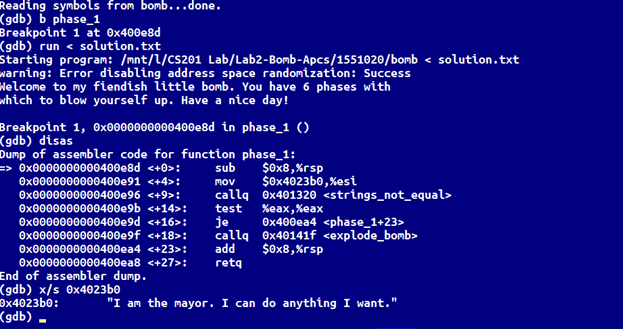
\includegraphics[width=\linewidth]{bai1.png}
  \caption{Phase1}
  \label{}
\end{figure}


\section{Phase2}

\paragraph{}
Set the breakpoint and jump into  \textless strings\_not\_equal\textgreater.
\newpage
\begin{figure}[h!]
  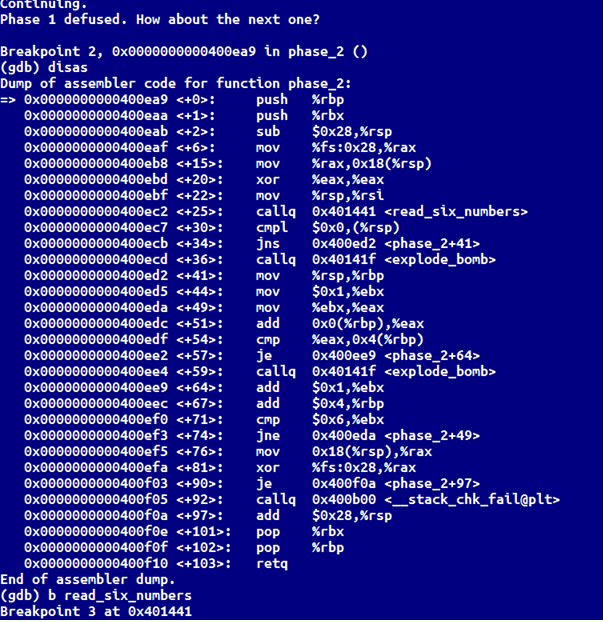
\includegraphics[width=\linewidth]{bai2_1.png}
  \caption{Phase 2}
  \label{}
\end{figure}

\paragraph{}
Here’s the assembly version of read six numbers.  
\newpage
\begin{figure}[h!]
  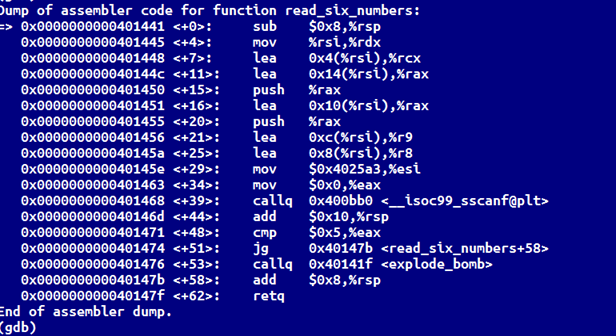
\includegraphics[width=\linewidth]{bai2_2.png}
  \caption{Phase 2.2}
  \label{}
\end{figure}


\paragraph{}
Nothing special, it just reads in 6 numbers. We continue looking at these steps  : 

\begin{figure}[h!]
  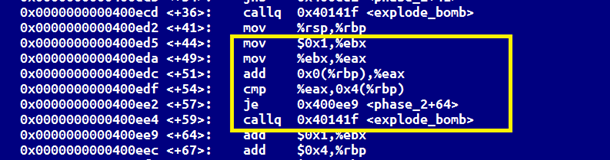
\includegraphics[width=\linewidth]{bai2_3.png}
  \caption{Phase 2.3}
  \label{}
\end{figure}

\paragraph{}
These codes tell us one important information. It means that when we add 1 with the first number we enter, if the result does not equal to the second number, we will die. So we have to make sure the second number = the first number + 1.  Let’s call the 1 here a “check” value. If you continue looking at the code, everything from 49 to 74 is a loop. Moreover, this loop goes through the 6 numbers we enter. Keep an eye on the change of ebx and rbp, we can conclude that after everyturn, the “check” value got raised by 1, the current number will move to the next number. Thus, the pattern for our inputted 6 numbers is :  \textless (N+1) position \textgreater number = \textless (N) position \textgreater number + check ( check runs from 1-5). At last, the result is 1 2 4 7 11 16 

\begin{figure}[h!]
  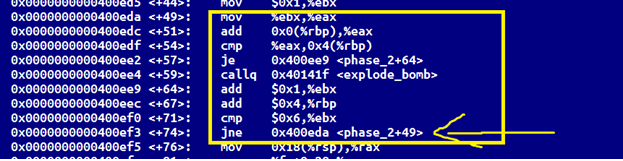
\includegraphics[width=\linewidth]{bai2_4.png}
  \caption{Phase 2.4}
  \label{}
\end{figure}

\newpage
\section{Phase3}

\paragraph{}
Here's the assembly code of phase\_3 : 
\newpage
\begin{figure}[h!]
  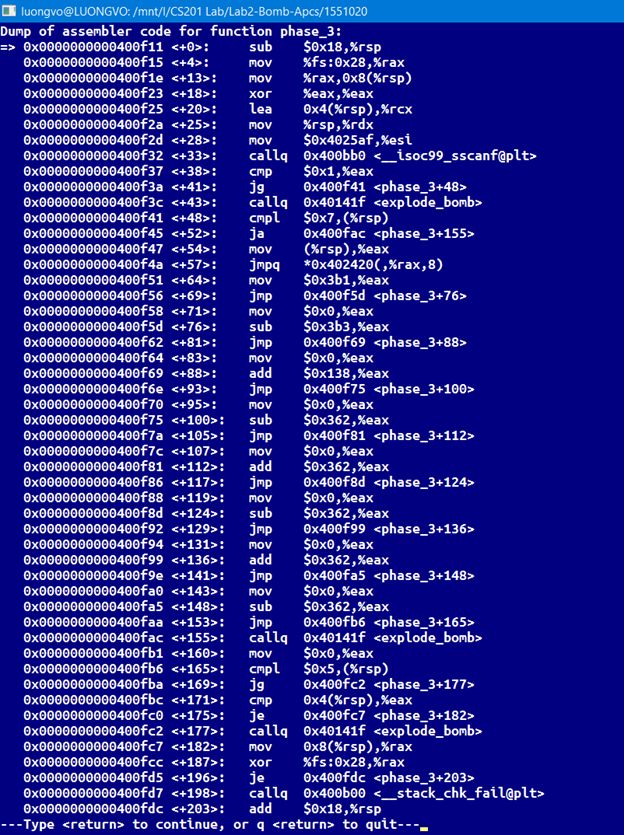
\includegraphics[height=0.7\textheight]{bai3_1.png}
  \caption{Phase 3.1}
  \label{}
\end{figure}

\paragraph{}
This lines tells  that we must have more than 1 input  : 
\newpage
\begin{figure}[h!]
  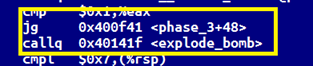
\includegraphics[width=\linewidth]{bai3_2.png}
  \caption{Phase 3.2}
  \label{}
\end{figure}


\paragraph{}
Now let's split the remaining lines into 3 parts, in which only 1 part we do care about. 

\begin{figure}[h!]
  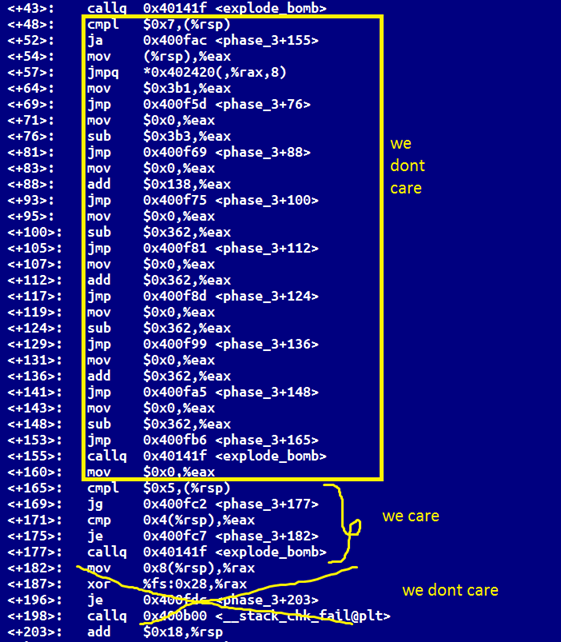
\includegraphics[width=\linewidth]{bai3_3.png}
  \caption{Phase 3.3}
  \label{}
\end{figure}

\paragraph{}
Why we don't care the first part. Because it's jump command everywhere. Eventually, it will end up at \textless +165\textgreater we don't have to worry at all. Now look at the part that we care. Obviously, if rsp \textgreater 5 then boom, it jumps to the bomb. So our first inputted number must be \textless=5.  Then we compare the next inputted number with eax ( which is 0 because of "mov 0x0, eax"). If the second inputted number is not equal to 0 then boom again as it will call the explode\_bomb. Therefore, my inputted solution is "4 0". 


\section{Phase4}

\paragraph{}
Here is the assembly code of Phase\_4 : 

\begin{figure}[h!]
  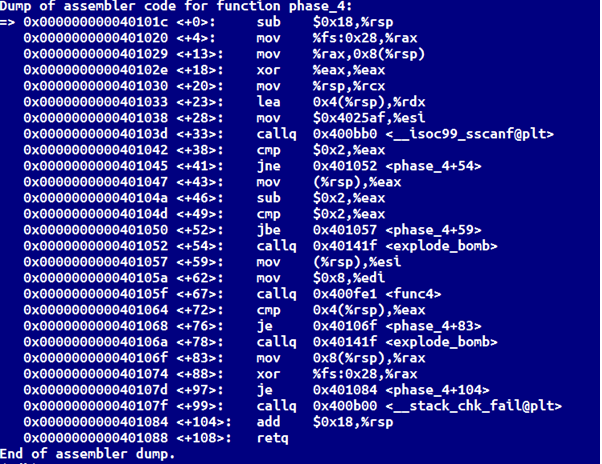
\includegraphics[width=\linewidth]{bai4_1.png}
  \caption{Phase 4.1}
  \label{}
\end{figure}

\paragraph{}
Firstly, this part here tells us that we should have 2 inputted numbers or the bomb will explode. Also, the inputted number must be smaller or equal to 4.
\newpage
\begin{figure}[h!]
  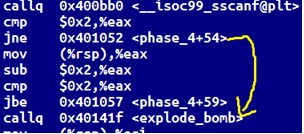
\includegraphics[width=\linewidth]{bai4_2.png}
  \caption{Phase 4.2}
  \label{}
\end{figure}

\paragraph{}
Then look at line \textless +67\textgreater, it calls func4 so we need to disassemble func4 code to see what it is doing inside.

\begin{figure}[h!]
  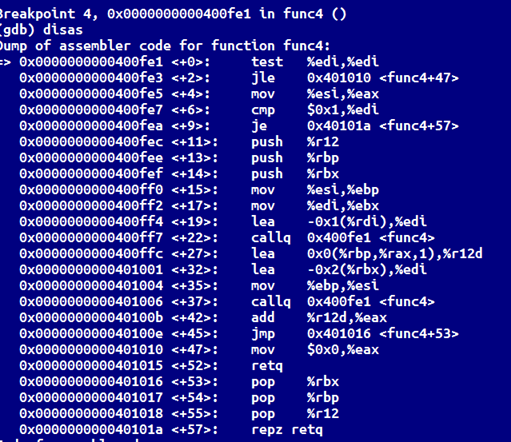
\includegraphics[width=\linewidth]{bai4_3.png}
  \caption{Phase 4.3}
  \label{}
\end{figure}

\paragraph{}
Some important informations about this func4 is that it is a recursion ( as on line \textless +22\textgreater  it is trying to call itself ) and all it does is adding to our first inputted number an equal value for 53 times then check if it matches the second inputted number. In short, 54 times multiply the first number must equals to the second number.  ( and don't forget the first inputted number must \textless=4 ).  

After func4, this block here shows that the program try to compare the second inputted number with the result of func4 ( which is the first inputted number mutiplied  by 54 times. 

\begin{figure}[h!]
  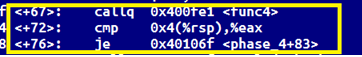
\includegraphics[width=\linewidth]{bai4_4.png}
  \caption{Phase 4.4}
  \label{}
\end{figure}
\paragraph{} Therefore the result is 162 3

\section{Phase5}

\paragraph{}
Here's the assembly code of phase\_5 

\begin{figure}[h!]
  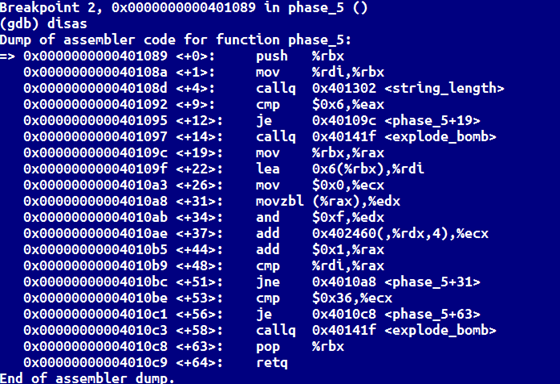
\includegraphics[width=\linewidth]{bai5_1.png}
  \caption{Phase 5.1}
  \label{}
\end{figure}


\paragraph{}
Clearly, we can see that it does something in the \textless string\_length\textgreater function. If the return of that function is smaller than 6 or bigger than 6, then the callq on \textless +14\textgreater will execute, which leads to the bomb. Therefore, we predict that we must enter a string with 6 numbers. Take a closer look into string\_length : 

\begin{figure}[h!]
  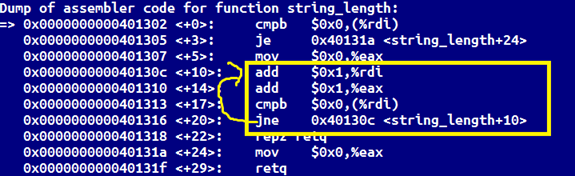
\includegraphics[width=\linewidth]{bai5_2.png}
  \caption{Phase 5.2}
  \label{}
\end{figure}


\paragraph{}
From line 10 to line 20, it is trying to do a loop in which it checks if the string length is equal to 6. Nothing special here.\newline
Now we proceed to the next important block . We can detect a loop at \textless +31\textgreater 

\begin{figure}[h!]
  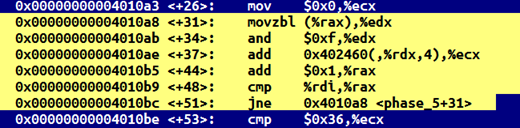
\includegraphics[width=\linewidth]{bai5_3.png}
  \caption{Phase 5.3}
  \label{}
\end{figure}


\paragraph{}
We notice that the loop tries to accomplish something with ecx since it is the address that doesn't move but keep being added up. 

\begin{figure}[h!]
  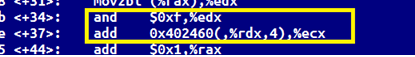
\includegraphics[width=\linewidth]{bai5_4.png}
  \caption{Phase 5.4}
  \label{}
\end{figure}

\paragraph{}
After some investigations, we will discover rax is the first element in our inputted string and rdi is the last element in our inputed string. ( I inputted 123456, 49 to 54 is their elements' ascii code).
\newpage
\begin{figure}[h!]
  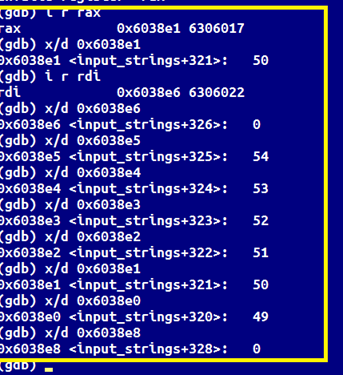
\includegraphics[width=\linewidth]{bai5_5.png}
  \caption{Phase 5.5}
  \label{}
\end{figure}

\paragraph{}
Also, by looking deeply in how rdx and rax change, we can conclude that the loop tries to change the address of eax.  
Now look at this . 

\begin{figure}[h!]
  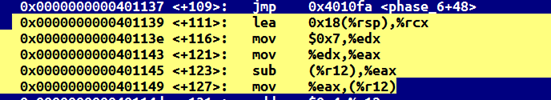
\includegraphics[width=\linewidth]{bai5_6.png}
  \caption{Phase 5.6}
  \label{}
\end{figure}

\paragraph{}
\begin{figure}[h!]
  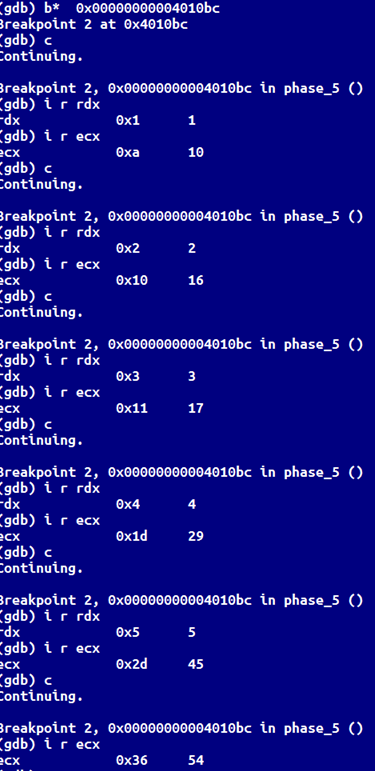
\includegraphics[height=0.8\textheight]{bai5_7.png}
  \caption{Phase 5.7}
  \label{}
\end{figure}


\paragraph{}
\newpage
But how much do we need to change eax ?  It's 54 in decimal or 36 in hexadecimal. Therefore, my input "123456" meets the requirement.
\begin{figure}[h!]
  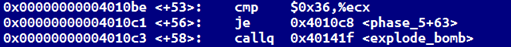
\includegraphics[width=\linewidth]{bai5_8.png}
  \caption{Phase 5.8}
  \label{}
\end{figure}

\section{Phase6}
 

\paragraph{}
Phase 6's assembly code is too long to be put all in here. Let's just dig into some important parts only.
At first glance, the program begins to read in 6 numbers we inputed. 


\begin{figure}[h!]
  
\includegraphics[width=\linewidth]{bai6_1.png}
  \caption{Phase 6.1}
  \label{}
\end{figure}

\paragraph{}
This loops tell us that the input must be 6 distinct numbers and smaller or equal to 6. So that's 1 2 3 4 5 6. 

\begin{figure}[h!]
  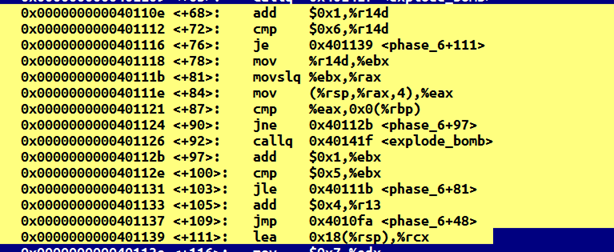
\includegraphics[width=\linewidth]{bai6_2.png}
  \caption{Phase 6.2}
  \label{}
\end{figure}

\paragraph{}
These lines here told us that the code subtract our inputted number by 7, then use the new value. After that these lines here  


\begin{figure}[h!]
  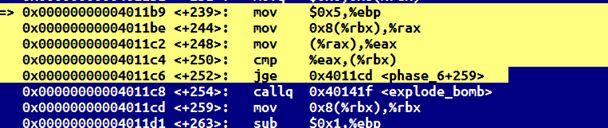
\includegraphics[width=\linewidth]{bai6_3.png}
  \caption{Phase 6.3}
  \label{}
\end{figure}

\paragraph{}
Told us that they are using the new values to compare. If these new values ( 7 - each inputted number ) follows ascending order, it would be fine. ( which means that our input must be in ascending order). 
However it is not as simple as 1 2 3 4 5 6. Every number got their own code so we got to use x/gx + address to decode all the number.  For example : 

\begin{figure}[h!]
  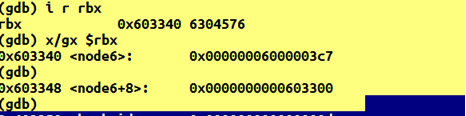
\includegraphics[width=\linewidth]{bai6_4.png}
  \caption{Phase 6.4}
  \label{}
\end{figure}

\paragraph{}
Rbx is the way to all the inputted number, so we use x/gx to find out the address of each member in it. Firstly, it is x/gx \$rbx. Here we have <node6> is the hex value of 6. And Node 6+8 is the address of the next node. Keep doing that and we will find the next node hex value and the next next node . 

\begin{figure}[h!]
  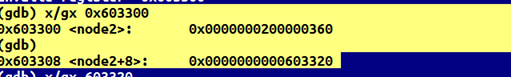
\includegraphics[width=\linewidth]{bai6_5.png}
  \caption{Phase 6.5}
  \label{}
\end{figure}

\paragraph{}
After all, sort all the hex value and rearrange the input .
We get the answer 1 5 3 6 2 4



\clearpage



\end{document}






